% !TEX root = 99_main.tex

\begin{figure}
\begin{center}
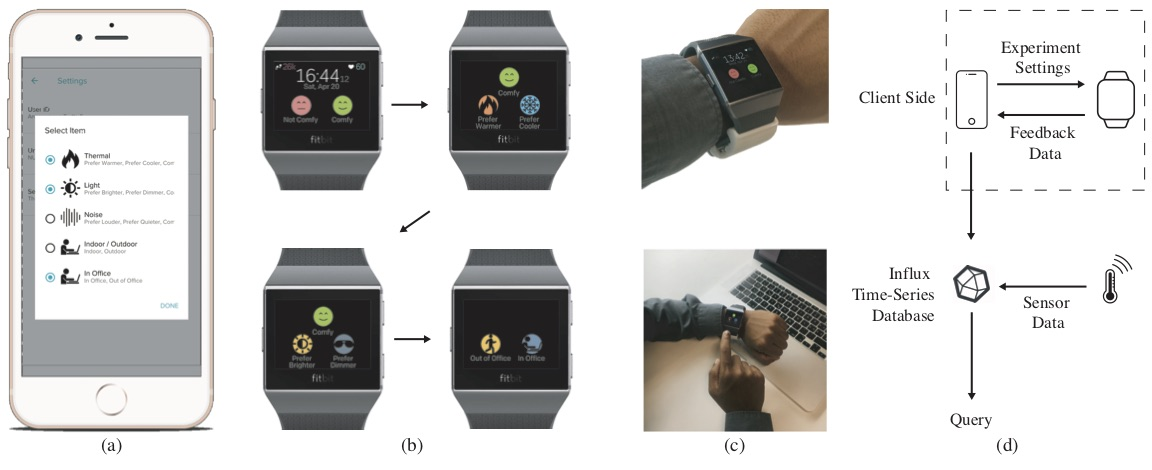
\includegraphics[width=\textwidth, trim= 0cm 0cm 0cm 0cm,clip]{cozie-overview.pdf}
\caption{Overview of the cozie app. (a) the fitbit mobile app is used to set experimental settings, (b) the flow of questions based on settings selected in (a), (c) photos of the watch-face in action with the strap-pack sensor box, (d) overview of data communication.}
\label{fig:homescreen}
\end{center}
\end{figure}

In the Ma\={o}ri legends of old, there was a time when the sun would travel quickly across the sky, leaving people without sufficient light and warmth. M\={a}ui, a great hero of the time, observed this discomfort amongst the village and went on a quest to tame the sun. Armed with his magic jawbone of Murirangawhenua and a lot of flax rope, he succeeded in tying down the sun and beating it, until it slowed down to the speeds we have today. What M\={a}ui effectively did was categorise everyone in a one-size-fits-all model, and based on this assumption, took action to change the environment he lived in. 

The way we control our buildings today, is similar to the way that M\={a}ui tamed the sun. We make an assumption of the general population based on a survey of a few people, and change the environment we live in based on these few data points. The issue here is that we assume that all occupants within a building zone share the same comfort preferences. In reality, variations in metabolic rates, light preferences, and noise tolerances presents a challenge when attempting to condition a work space to meet the requirements of all occupants. 

However understanding the preferences of individuals presents a significant challenge, both the times of M\={a}ui and now. The state of the art of human comfort data collection is in the form of surveys, either as an online form, or paper based. While this in principal works, it presents three major challenges.

% %A recent survey of 52'980 occupants in 251 office buildings found that 50\% of all occupants were dissatisfied with their indoor environment. 


% From the times of M\={a}ui till now, a significant challenge is the acquisition of human comfort feedback data. The state of the art, in attaining human feedback are surveys, either as an online form, or paper based. 

\begin{itemize}
  \item The methodology cannot be scaled to large sample sets due to the administrative overhead in preparing these studies.
  \item The studies are often conducted outside of the test subjects natural working environment.
  \item Users suffer from survey fatigue \cite{porter2004multiple} due to the number of data points required to conduct a thorough assessment. Even when willing to participate, there is a concern about how accurately their responses are \cite{Clear2018}.
\end{itemize}



This paper presents cozie, a publicly available clock-face designed for fitbit which can be used for tailored, scalable, in-situ human comfort studies. We will show how the watch-face can be deployed for a range of tailored experimental scenarios, and be evaluated using modern data analytics to infer behavioral patterns of the test participants. This information can be used to optimise human comfort through spatial recommendation, or combined with building sensor data to create a labeled data-set for the comfort optimisation of the building management system. \\

% combined with building sensor data to create a high quality labeled data set. 


%  that can be used to optimise the comfort of the user through spatial recommendation, and provide input training data for the comfort optimisation of the building management system.\\

The remainder of the paper is organised as follows. The next section outlines the cozie clock-face and how research teams can implement it for a variety of human comfort related experiments. In Section 3 we detail a preliminary experiment conducted using the cozie clock-face for building comfort optimisation, Section 4 presents the preliminary results from this experiment, and Section 5 discusses our findings and next steps in this project. Finally, Section 6 concludes the paper. 





% \begin{figure}
% \begin{center}
% \includegraphics[width=8cm, trim= 0cm 0cm 0cm 0cm,clip]{facadeFunctionsnew.pdf}
% \caption{The facade acting as a mediator between the interior and exterior environment, while fulfilling various functions \cite{nagy2016adaptive}}
% \label{fig:ASFschematic}
% \end{center}
% \end{figure}

% \begin{figure}
% \begin{center}
% \includegraphics[width=8cm, trim= 0cm 0cm 0cm 0cm,clip]{honr.jpg}
% \caption{An example of an ASF constructed at the House of Natural Resources \cite{nagy2016adaptive}}
% \label{fig:HoNR}
% \end{center}
% \end{figure}




